\documentclass[10pt]{beamer}

\usetheme[progressbar=frametitle]{m}

\usepackage{booktabs}
\usepackage[scale=2]{ccicons}
\usepackage{mathtools}
\usepackage[]{mcode}

\usepackage{listings}             % Include the listings-package
\lstset{ % General setup for the package
	language=Perl,
	basicstyle=\small\sffamily,
	numbers=left,
 	numberstyle=\tiny,
	frame=tb,
	tabsize=4,
	columns=fixed,
	showstringspaces=false,
	showtabs=false,
	keepspaces,
	commentstyle=\color{red},
	keywordstyle=\color{blue}
}

%\usepackage{pgfplots}
%\usepgfplotslibrary{dateplot}

\title{Análisis de Resursos MPI en BIOMED}
\date{8 Abril 2016}
\author{Mihaita Alexandru Lupoiu}
\institute{Modelos de Programación en Grid (Mpg)}
\titlegraphic{\hfill
\includegraphics[height=2.0cm]{logo.png}}

\begin{document}

\maketitle
%-------------------------------------------------------------------------------------------%
\begin{frame}
  \frametitle{Trabajo propuesto}
  \setbeamertemplate{section in toc}[sections numbered]
  \tableofcontents[hideallsubsections]
\end{frame}
%-------------------------------------------------------------------------------------------%
\section{Introdución}
%-------------------------------------------------------------------------------------------%
\begin{frame}[fragile]
  \frametitle{Introdución}
  
  El objetivo de este proyecto es analizar los recursos MPI de Biomed. Para ellos se van a analizar los recursos mediante:
  
\begin{itemize}
\item El análisis del retardo que existe a la hora de enviar un mensaje mediante el programa Ping Pong.
\item El análisis del rendimiento de una aplicación que tiene un coste computacional importante y además que tiene dependencia de datos.
\end{itemize}
  
\end{frame}
%-------------------------------------------------------------------------------------------%
\begin{frame}[fragile]
\frametitle{Introdución}

La aplicación que tiene un coste computacional importante es la la factorización \textsc{LDL'}, que es una forma de factorización de una matriz \textsc{A} como el producto de una matriz triangular inferior \textsc{L} por una diagonal \textsc{D} y por una matriz inferior traspuesta \textsc{L'}.

  \begin{equation*}
    A = L*D*L^T
  \end{equation*}

  Para evitar conplicaciones las pruebas se harán solo para matrices simétricas, eso significa que \textsc{A = A'}.
\end{frame}

%-------------------------------------------------------------------------------------------%
\section{Ejemplo LDL'}
%-------------------------------------------------------------------------------------------%
\begin{frame}[fragile]

\frametitle{Ejemplo LDL'} 
Ejemplo sin sobre-escritura:

\[
A=
  \begin{bmatrix}
    4 & 3 & 1 & 1 \\
    3 & 8 & 1 & 2 \\
    1 & 1 & 16 & 1 \\
    1 & 2 & 1 & 10 \\
  \end{bmatrix}
\]

\[
\underbracket[0pt][0pt]{%
\begin{bmatrix}
    1 & 0 & 0 & 0 \\
    0.75 & 1 & 0 & 0 \\
    0.25 & 0.0435 & 1 & 0 \\
    0.25 & 0.2174 & 0.0442 & 1 \\
\end{bmatrix}}_{\mathstrut L}
\times
\underbracket[0pt][0pt]{%
\begin{bmatrix}
    4\\
    5,75\\
    15.7391\\
    9.4475\\
\end{bmatrix}}_{\mathstrut D}
\times
\underbracket[0pt][0pt]{%
\begin{bmatrix}
	1 & 0.75 & 0.25 & 0.25 \\
    0 & 1 & 0.0435 & 0.2174 \\
    0 & 0 & 1 & 0.0442 \\
    0 & 0 & 0 & 1 \\
\end{bmatrix}}_{\mathstrut L'}
\]

\end{frame}
%-------------------------------------------------------------------------------------------%
\begin{frame}[fragile]

\frametitle{Ejemplo LDL'} 
Ejemplo con sobre-escritura:

\[
A=
  \begin{bmatrix}
    4 & 3 & 1 & 1 \\
    3 & 8 & 1 & 2 \\
    1 & 1 & 16 & 1 \\
    1 & 2 & 1 & 10 \\
  \end{bmatrix}
\]

\[
LDL'=
  \begin{bmatrix}
    4 & 0 & 0 & 0 \\
    0.75 & 5,75 & 0 & 0 \\
    0.25 & 0.0435 & 15.7391 & 0 \\
    0.25 & 0.2174 & 0.0442 & 9.4475 \\
  \end{bmatrix}
\]

\end{frame}
%-------------------------------------------------------------------------------------------%
\section{Configuración}
%-------------------------------------------------------------------------------------------%
\begin{frame}[fragile]
\frametitle{Configuración}

	Para el lanzamiento de la aplicación en BIOMED se tienen que crear varios ficheros:
    
\begin{enumerate}
\item El fichero de pre configuración ''pre-hook.sh'' que se encargará de compilar el programa en la máquina remota, copiar ficheros necesarios, etc.
\item El fichero de ''start.sh'', para que se puedan utilizar distintas versiones de MPI. En este caso se utiliza el mismo que se utilizó en las practicas.
\item El fichero ''program.jdl'' que se encarga de especificar los requisitos de la aplicación para que se pueda ejecutar con exito.
\item El fichero de post configuración ''post-hook.sh'' que se encargará de realizar el procesado de los resultados de la aplicación en caso de que sea necesario. En este caso no lo es.
\end{enumerate}
\end{frame}
%-------------------------------------------------------------------------------------------%
\begin{frame}[fragile]
\frametitle{Configuración}
	El fichero de configuración en este caso es el siguiente:
\begin{lstlisting}[basicstyle=\ttfamily]
#!/bin/sh
pre_run_hook () {
    tar xzvf file.tar.gz
    make 
	
    return 0
}
\end{lstlisting}

Dentro de ''file.tar.gz'' está todo el código de la aplicación que se quiere lanzar y el makefile.

\end{frame}
%-------------------------------------------------------------------------------------------%
\begin{frame}[fragile]
\frametitle{Configuración}
    El fichero de los requisitos del sistema es el siguiente:
\begin{lstlisting}[basicstyle=\ttfamily\tiny]
JobType         = "Normal";
nodeNumber      = 4;
Executable      = "starter.sh";
Arguments       = "mpi.out OPENMPI";
InputSandbox    = {"starter.sh", "ldl.tar.gz", "pre-hook.sh"};
StdOutput       = "std.out";
StdError        = "std.err";
OutputSandbox   = {"std.out","std.err"};
Requirements    =
Member("MPI-START",other.GlueHostApplicationSoftwareRunTimeEnvironment)
&& Member("OPENMPI",other.GlueHostApplicationSoftwareRunTimeEnvironment)
&& Member("MPI-ETHERNET",other.GlueHostApplicationSoftwareRunTimeEnvironment);
Environment 	= {"I2G_MPI_PRE_RUN_HOOK=pre-hook.sh"};

\end{lstlisting}
\end{frame}
%-------------------------------------------------------------------------------------------%
\begin{frame}[fragile]
\frametitle{Configuración}

Los comandos utilizados fueron:
\begin{itemize}

\item Para listar los recursos donde se puede ejecutar la aplicación:
\begin{verbatim}
glite-wms-job-list-match -a program.jdl
\end{verbatim}

\item Para el envío del y arranque de la aplicación:
\begin{verbatim}
glite-wms-job-submit -a program.jdl
\end{verbatim}
\item Para cancelar una aplicación:
\begin{verbatim}
glite-wms-job-cancel  https://URL_submit
\end{verbatim}

\item Para la observar el estado de la aplicación:
\begin{verbatim}
glite-wms-job-status https://URL_submit
\end{verbatim}

\item Para recuperar la salida estándar  de la aplicación:
\begin{verbatim}
glite-wms-job-output --dir . https://URL_submit
\end{verbatim}

\end{itemize}

\end{frame}
%-------------------------------------------------------------------------------------------%
\section{Resultados Ping Pong}
%-------------------------------------------------------------------------------------------%
\begin{frame}[fragile]
\frametitle{Resultados: Tiempo empleado}
\begin{center}
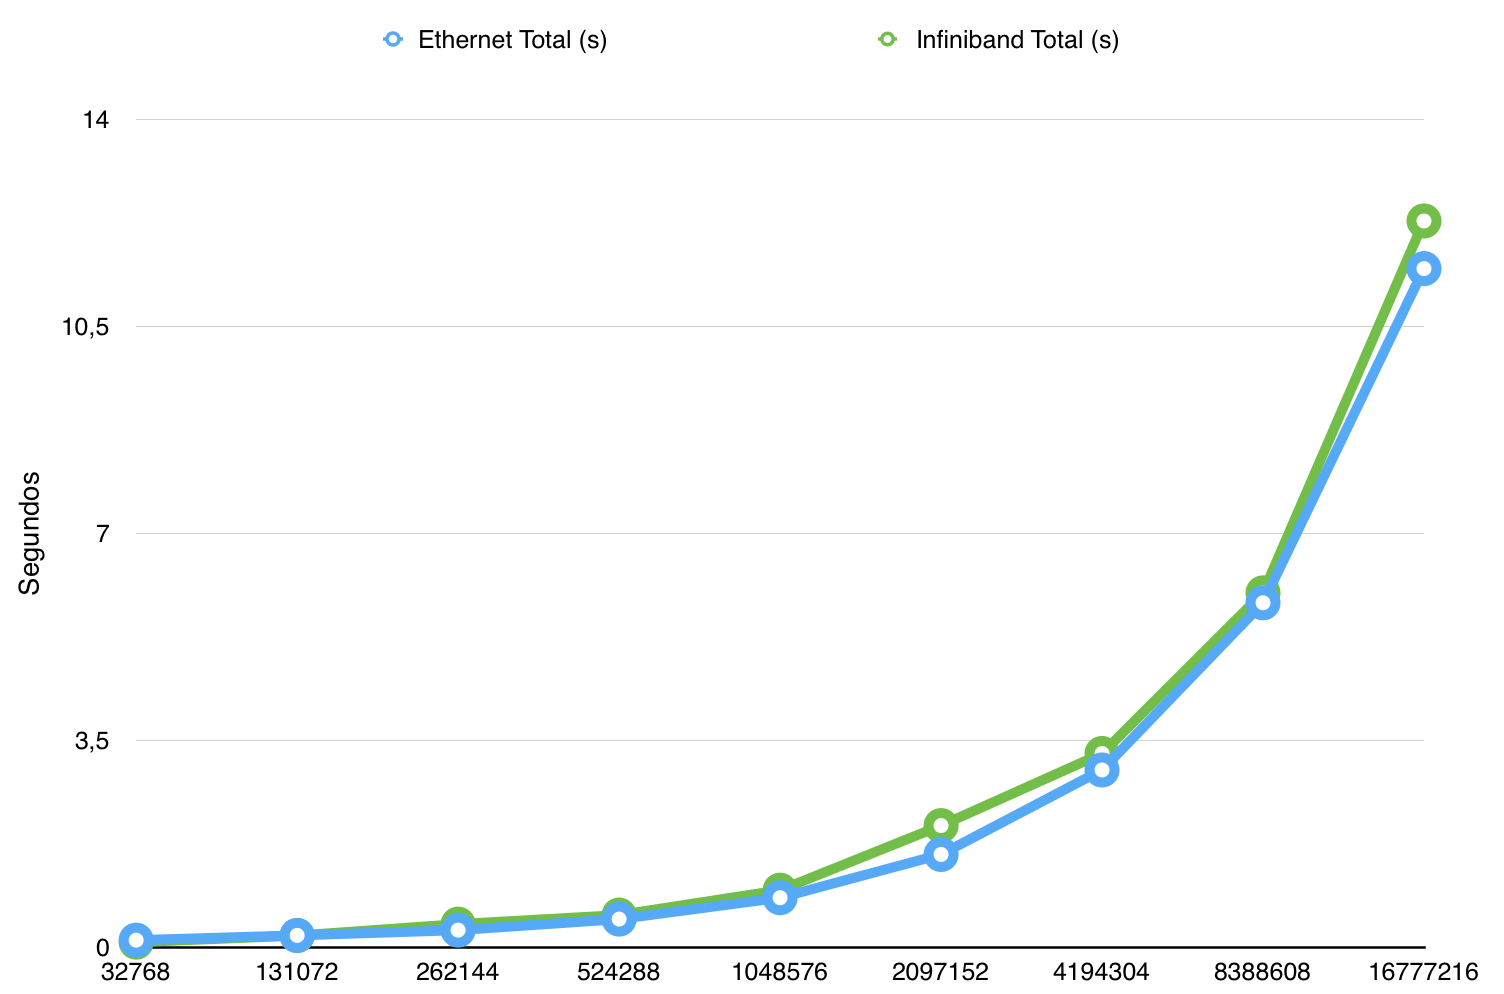
\includegraphics[scale=0.42]{1.png}
\end{center}
\end{frame}
%-------------------------------------------------------------------------------------------%
\begin{frame}[fragile]
\frametitle{Resultados: Tiempo/Envio (s) 4 KB}
\begin{center}
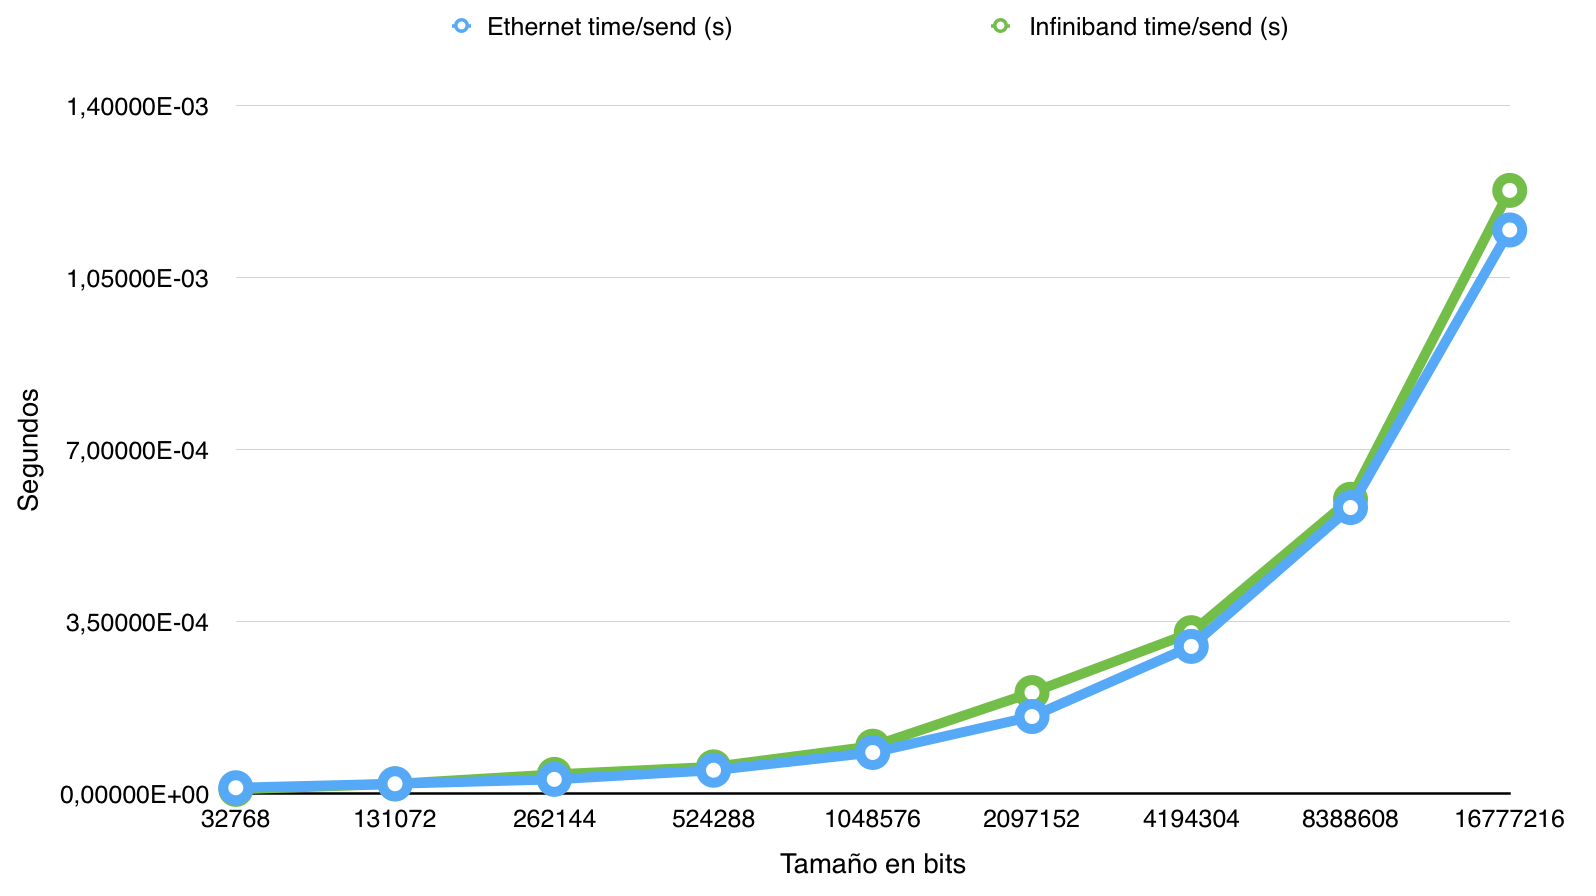
\includegraphics[scale=0.42]{2.png}
\end{center}
\end{frame}
%-------------------------------------------------------------------------------------------%
\begin{frame}[fragile]
\frametitle{Resultados: KB/s 4 KB}
\begin{center}
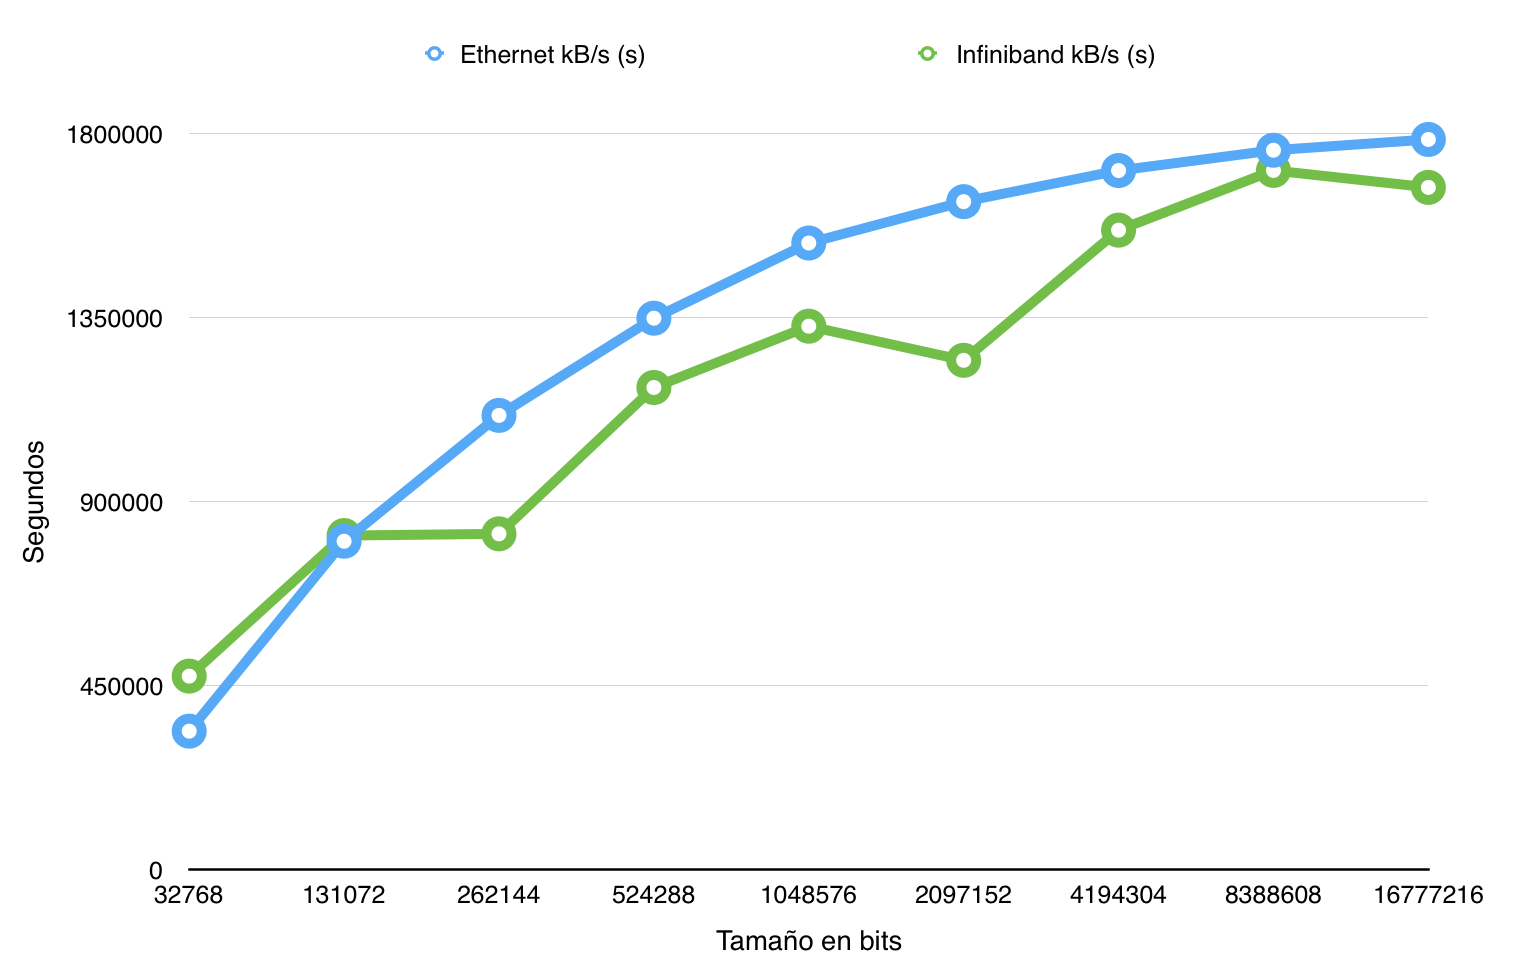
\includegraphics[scale=0.42]{3.png}
\end{center}
\end{frame}
%-------------------------------------------------------------------------------------------%
\begin{frame}[fragile]
\frametitle{Resultados: Tiempo empleado }
\begin{center}
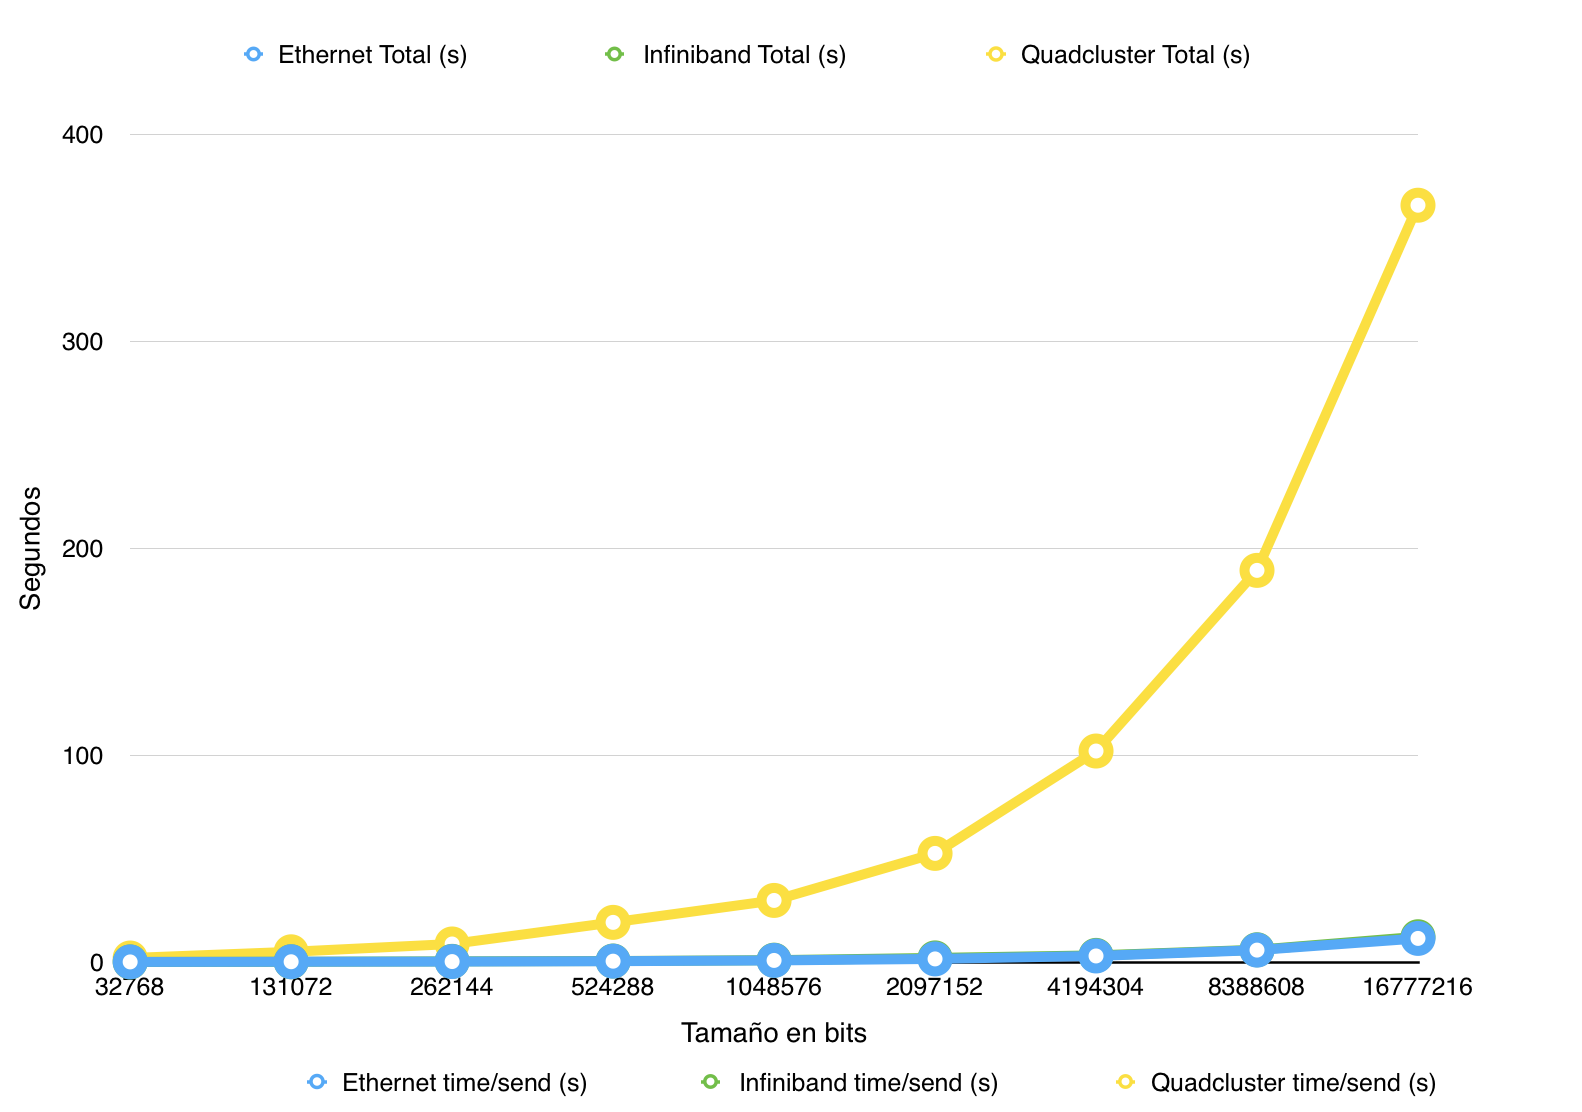
\includegraphics[scale=0.42]{4.png}
\end{center}
\end{frame}
%-------------------------------------------------------------------------------------------%
\begin{frame}[fragile]
\frametitle{Resultados: Tiempo/Envio (s) 128KB}
\begin{center}
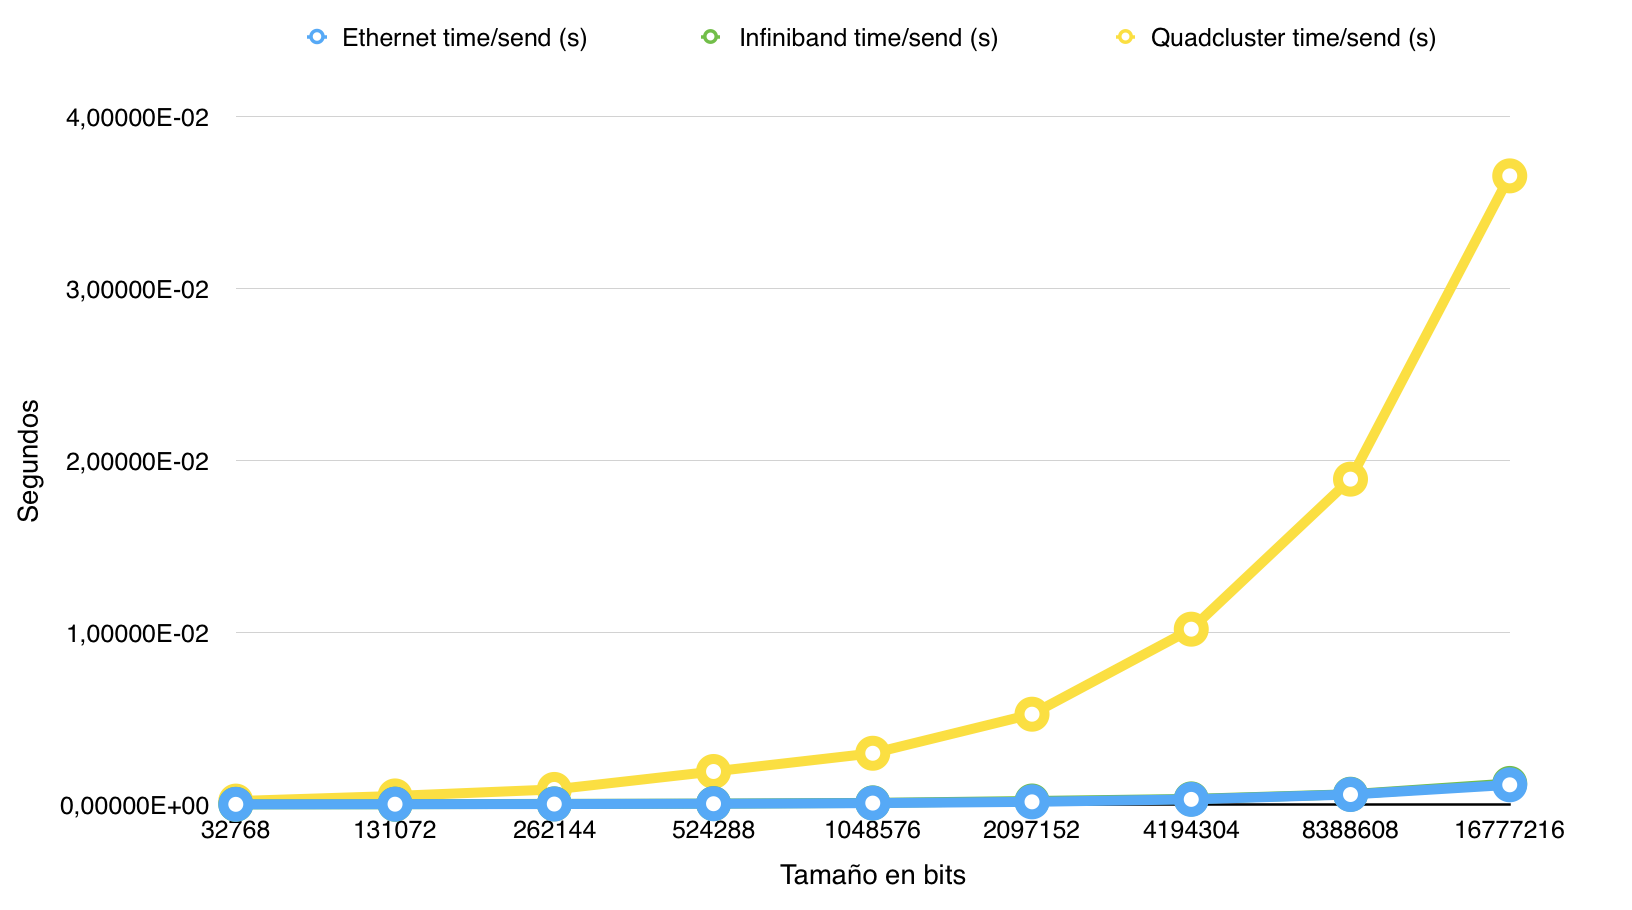
\includegraphics[scale=0.42]{5.png}
\end{center}
\end{frame}
%-------------------------------------------------------------------------------------------%
\begin{frame}[fragile]
\frametitle{Resultados: KB/s 128KB}
\begin{center}
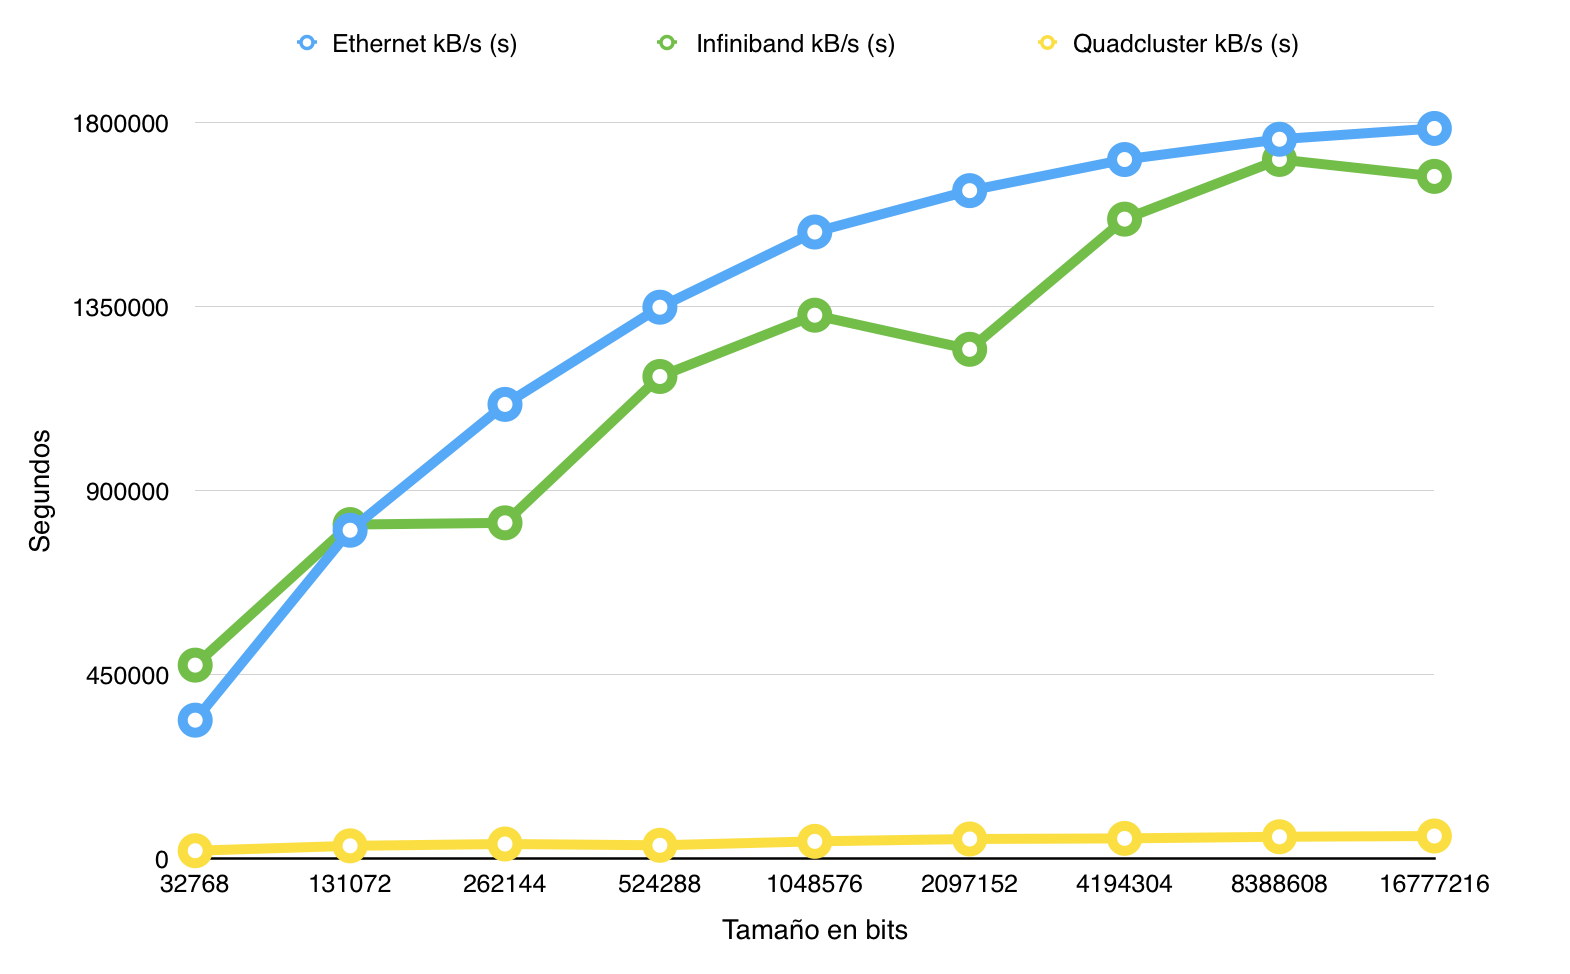
\includegraphics[scale=0.42]{6.png}
\end{center}
\end{frame}
%-------------------------------------------------------------------------------------------%
\section{Resultados LDL'}
%-------------------------------------------------------------------------------------------%
\begin{frame}[fragile]
\frametitle{Resultados: Matriz 4000x4000}
\begin{center}
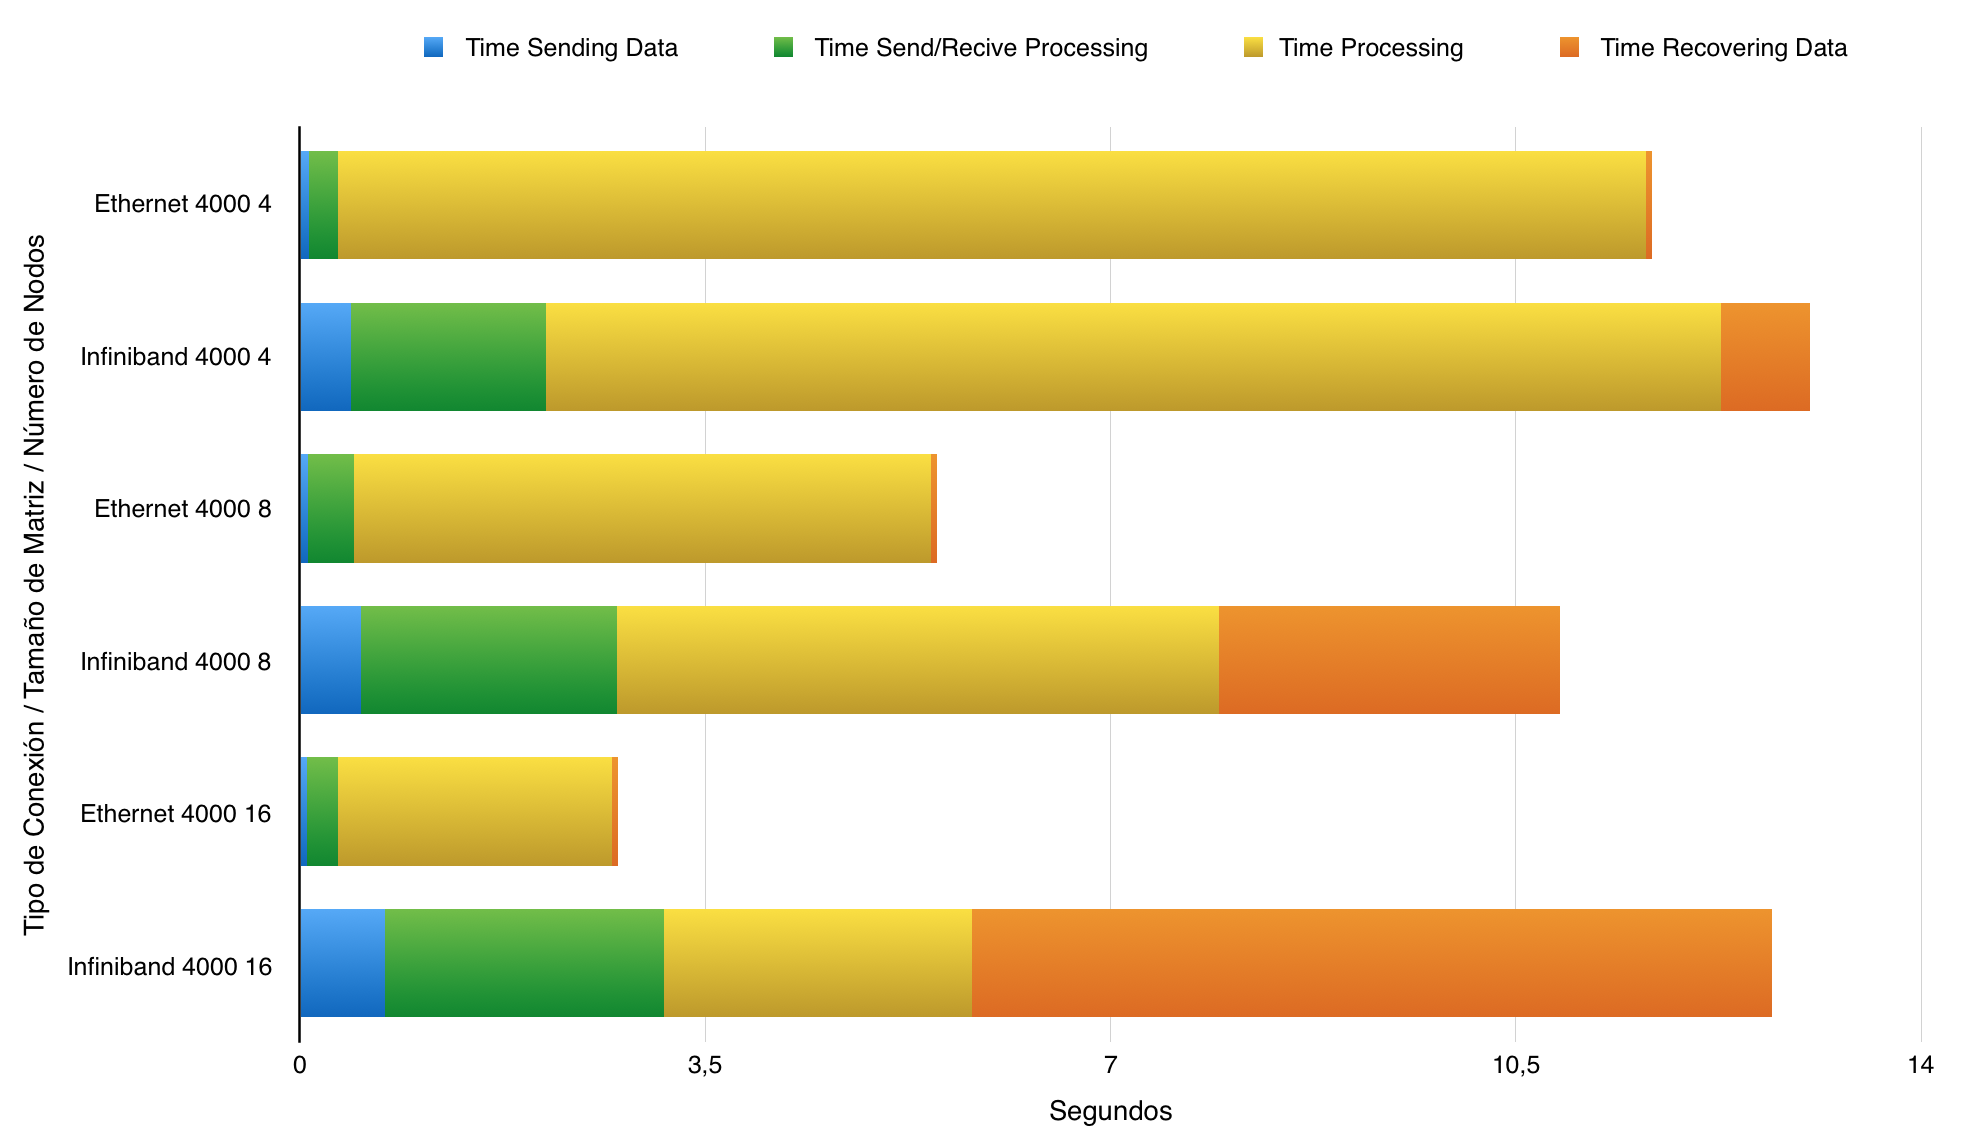
\includegraphics[scale=0.32]{4000.png}
\end{center}
\end{frame}
%-------------------------------------------------------------------------------------------%
\begin{frame}[fragile]
\frametitle{Resultados: Matriz 8000x8000}
\begin{center}
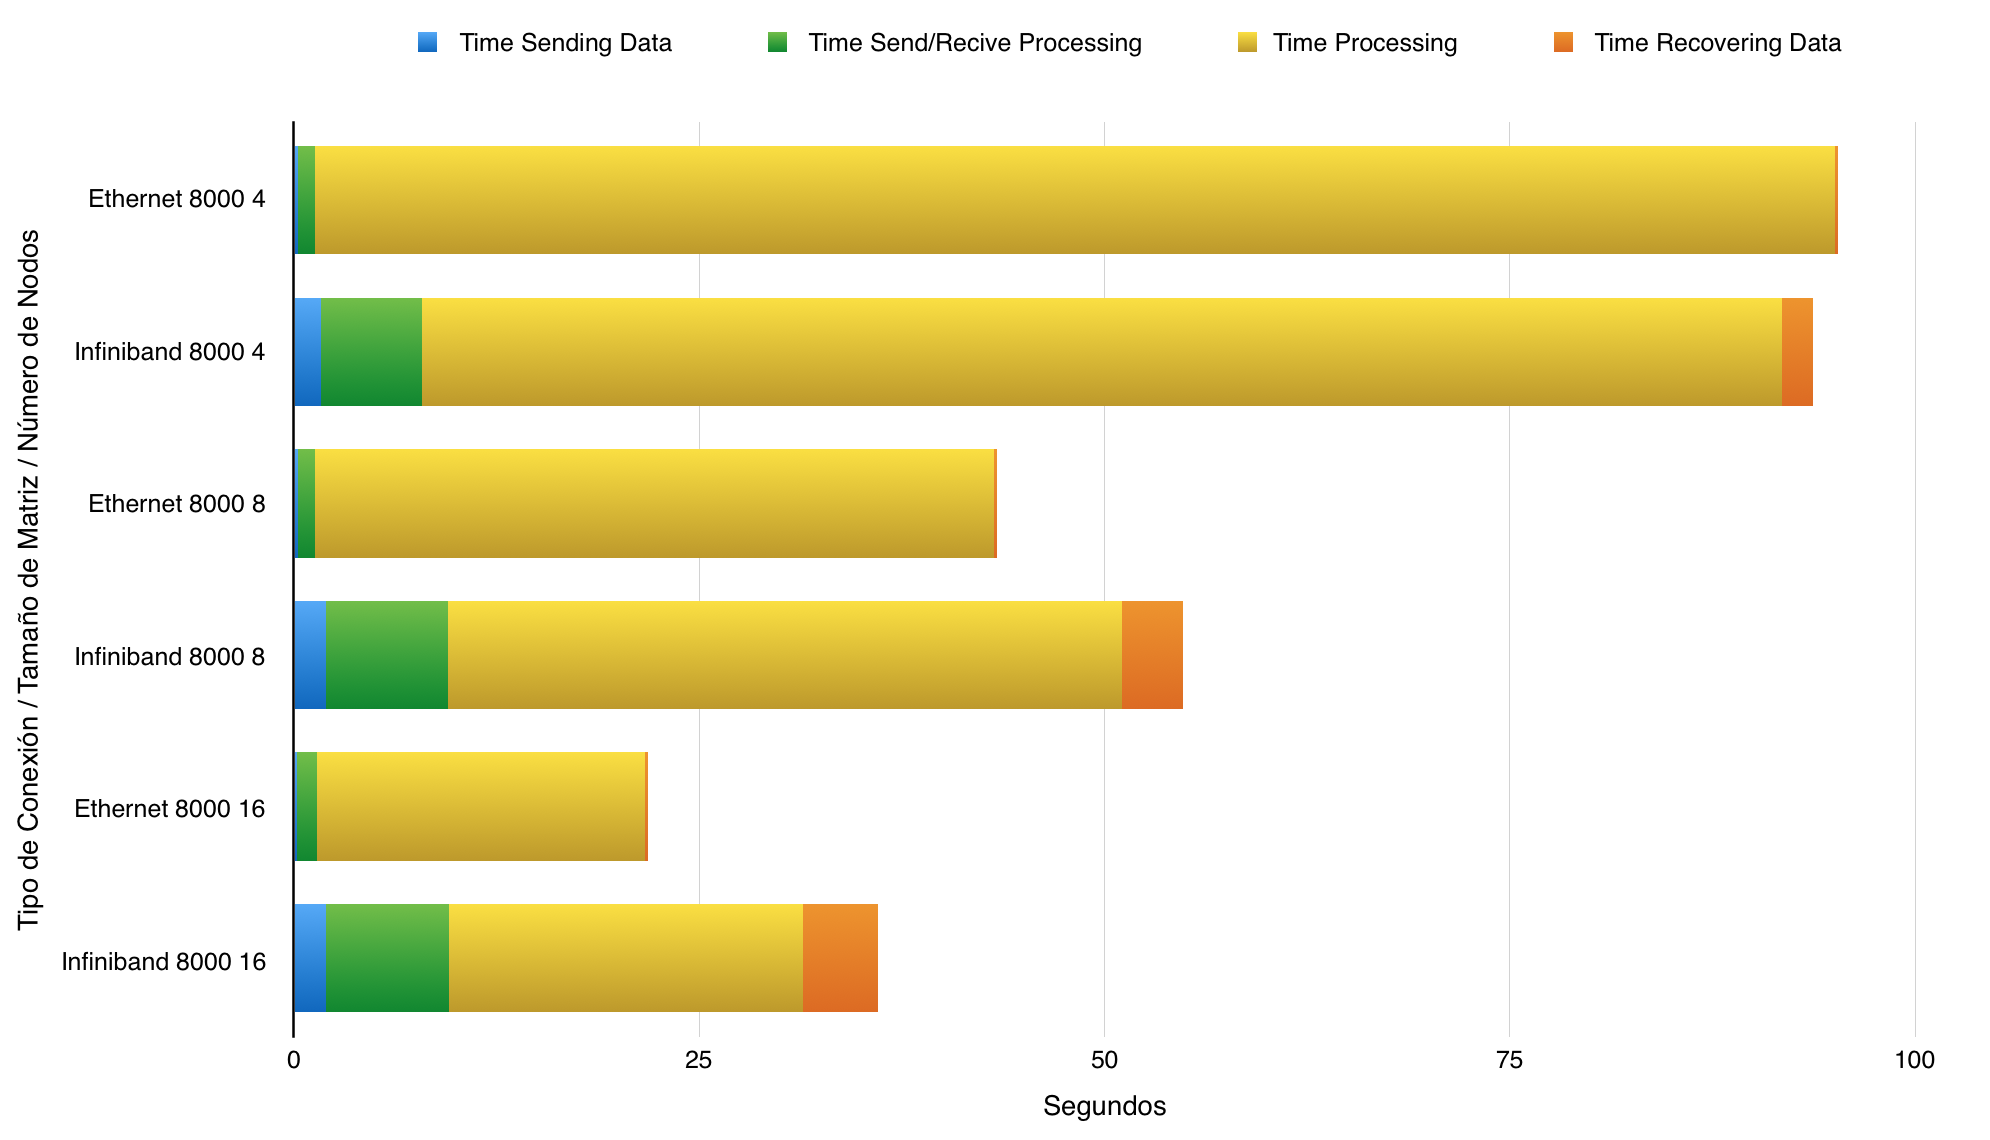
\includegraphics[scale=0.32]{8000.png}
\end{center}
\end{frame}
%-------------------------------------------------------------------------------------------%
\section{Conclusion y Trabajos Futuros}
%-------------------------------------------------------------------------------------------%
\begin{frame}{Conclusion y Trabajos Futuros}

  El algoritmo de la factorización $LDL^T$ implementar de manera concurrente y con unas mejoras considerables.\linebreak[2]

  Se ha podido observar que el claud computing de Azure puede ser una buena alternativa y mucho más barata para cálculos pesados si no se dispone de un equipo adecuado.\linebreak[2]


  Para futuras mejoras se debería de utilizar BLASH para la actualización de la matriz en MPI y utilizar un algoritmo por bloques para reducir las comunicaciones.
  
  Se debería de intentar realizar pruebas con más de 4 nodos de tipo D1 para ver cuando se puede conseguir de mejor, además se deberían de probar otros proveedores de cloud computing como Amazon para comparar sus servicios.
    
\end{frame}
%-------------------------------------------------------------------------------------------%
\section{Código}
%-------------------------------------------------------------------------------------------%
\begin{frame}{Código}

  Pueden conseguir todo el código fuente en
  \begin{center}\url{github.com/MihaiLupoiu/MPG}\end{center}

  Todo bajo la licencia
  \href{http://creativecommons.org/licenses/by-sa/4.0/}{Creative Commons
  Attribution-ShareAlike 4.0 International License}.

  \begin{center}\ccbysa\end{center}

\end{frame}
%-------------------------------------------------------------------------------------------%
\plain{¡Gracias!}
%-------------------------------------------------------------------------------------------%
\plain{¿Alguna pregunta?}
%-------------------------------------------------------------------------------------------%
\end{document}
